\hypertarget{_clip_8hpp}{
\subsection{Clip.hpp File Reference}
\label{_clip_8hpp}\index{Clip.hpp(166)@{Clip.hpp(166)}}
}
Declaration of \hyperlink{class_clip}{Clip} class.  


{\tt \#include $<$vector$>$}\par
{\tt \#include \char`\"{}NessieException.hpp\char`\"{}}\par


Include dependency graph for Clip.hpp:\nopagebreak
\begin{figure}[H]
\begin{center}
\leavevmode
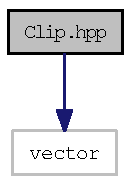
\includegraphics[width=121pt]{_clip_8hpp__incl}
\end{center}
\end{figure}


This graph shows which files directly or indirectly include this file:\nopagebreak
\begin{figure}[H]
\begin{center}
\leavevmode
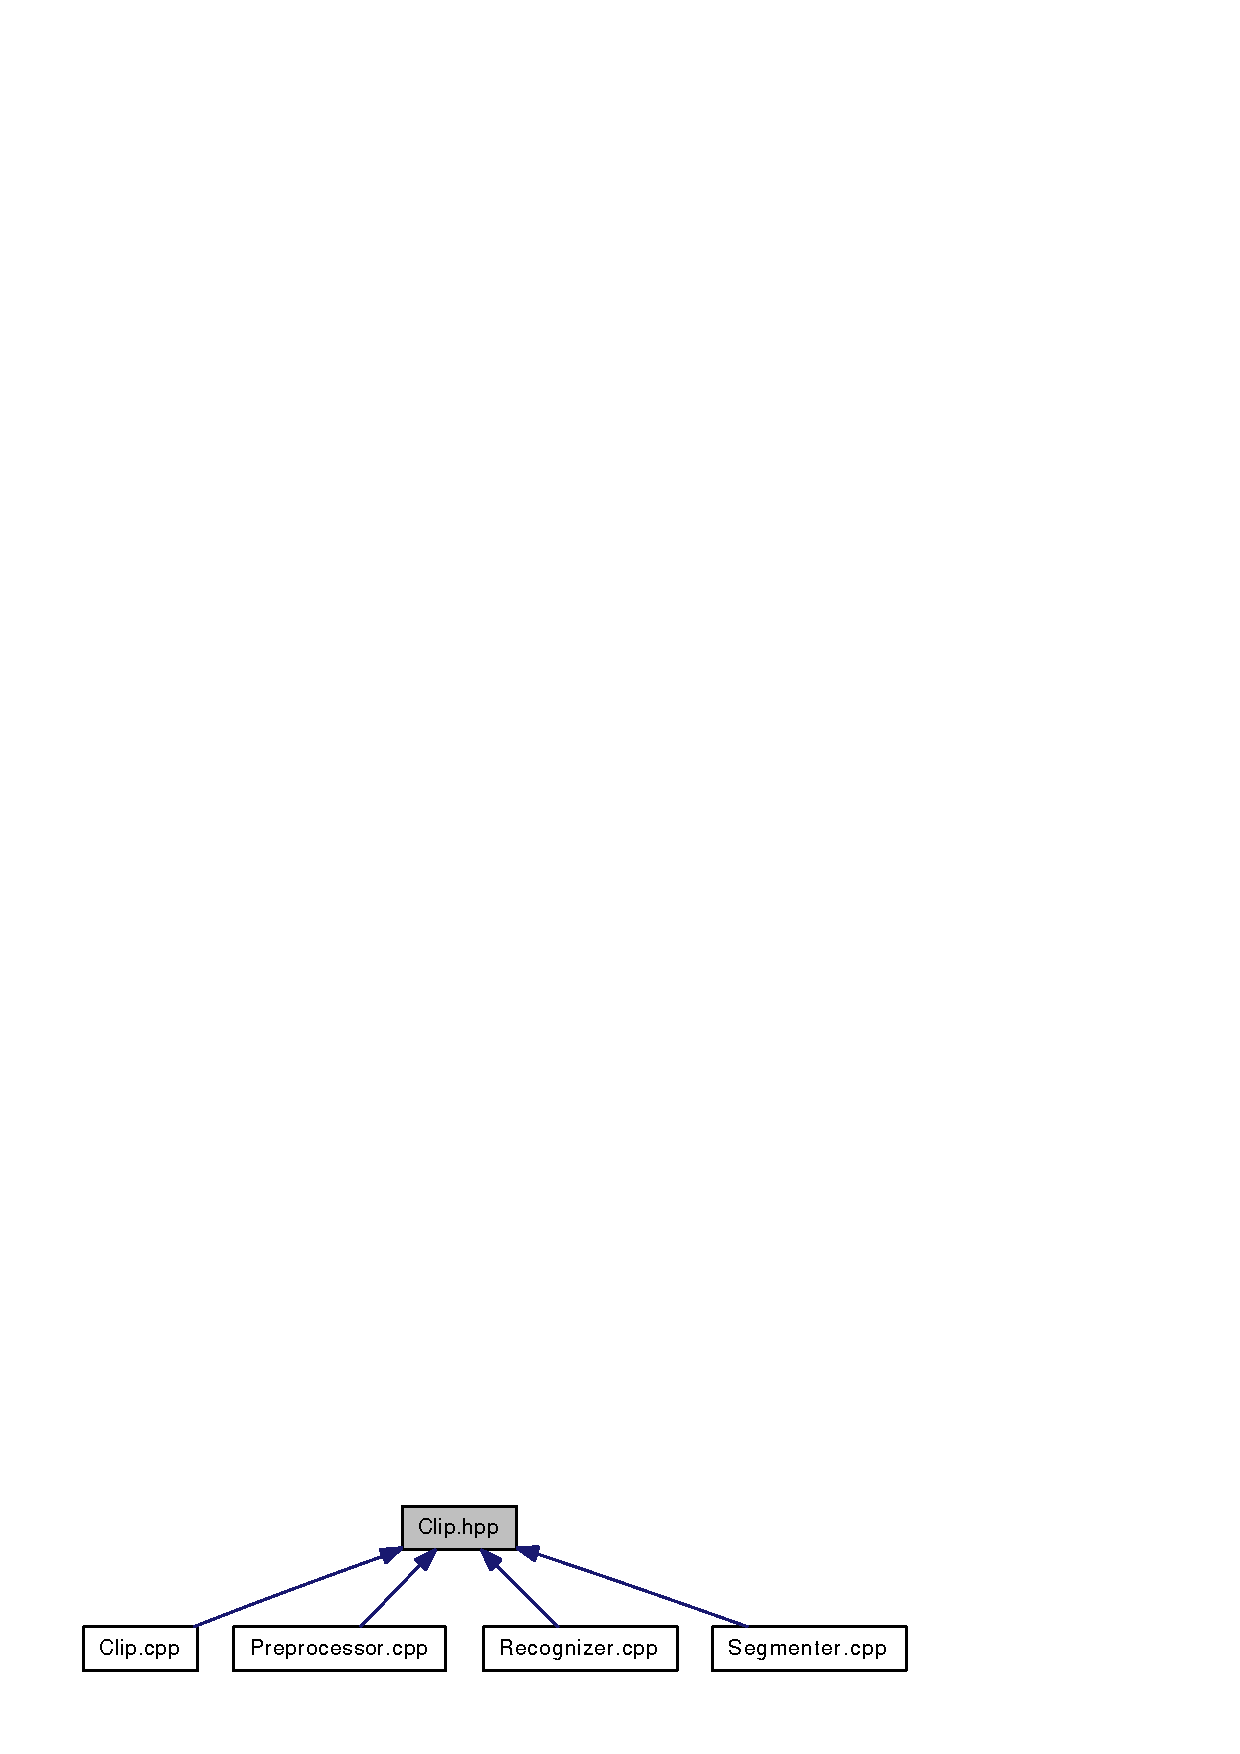
\includegraphics[width=219pt]{_clip_8hpp__dep__incl}
\end{center}
\end{figure}
\subsubsection*{Data Structures}
\begin{CompactItemize}
\item 
class \hyperlink{class_clip}{Clip}
\begin{CompactList}\small\item\em Press clip where the recognizer has to extract the text from. \item\end{CompactList}\end{CompactItemize}


\subsubsection{Detailed Description}
